%%%%%%%%%%%%%%%%%%%%%%%%%%%%%%%%%%%%%%%%%
%
% This template has been downloaded from:
% http://www.LaTeXTemplates.com
%
% License:
% CC BY-NC-SA 3.0 (http://creativecommons.org/licenses/by-nc-sa/3.0/)
%
%%%%%%%%%%%%%%%%%%%%%%%%%%%%%%%%%%%%%%%%%

%----------------------------------------------------------------------------------------
%	PACKAGES AND OTHER DOCUMENT CONFIGURATIONS
%----------------------------------------------------------------------------------------

\documentclass[final]{beamer}

\usepackage[scale=1.24]{beamerposter} % Use the beamerposter package for laying out the poster
\usepackage{caption}

\usetheme{confposter} % Use the confposter theme supplied with this template

\setbeamercolor{block title}{fg=ngreen,bg=white} % Colors of the block titles
\setbeamercolor{block body}{fg=black,bg=white} % Colors of the body of blocks
\setbeamercolor{block alerted title}{fg=white,bg=dblue!70} % Colors of the highlighted block titles
\setbeamercolor{block alerted body}{fg=black,bg=dblue!10} % Colors of the body of highlighted blocks
% Many more colors are available for use in beamerthemeconfposter.sty

%-----------------------------------------------------------
% Define the column widths and overall poster size
% To set effective sepwid, onecolwid and twocolwid values, first choose how many columns you want and how much separation you want between columns
% In this template, the separation width chosen is 0.024 of the paper width and a 4-column layout
% onecolwid should therefore be (1-(# of columns+1)*sepwid)/# of columns e.g. (1-(4+1)*0.024)/4 = 0.22
% Set twocolwid to be (2*onecolwid)+sepwid = 0.464
% Set threecolwid to be (3*onecolwid)+2*sepwid = 0.708

\newlength{\sepwid}
\newlength{\onecolwid}
\newlength{\twocolwid}
\newlength{\threecolwid}
\setlength{\paperwidth}{48in} % A0 width: 46.8in
\setlength{\paperheight}{36in} % A0 height: 33.1in
\setlength{\sepwid}{0.024\paperwidth} % Separation width (white space) between columns
\setlength{\onecolwid}{0.22\paperwidth} % Width of one column
\setlength{\twocolwid}{0.464\paperwidth} % Width of two columns
\setlength{\threecolwid}{0.708\paperwidth} % Width of three columns
\setlength{\topmargin}{-0.5in} % Reduce the top margin size
%-----------------------------------------------------------

\usepackage{graphicx}  % Required for including images

\usepackage{booktabs} % Top and bottom rules for tables

%----------------------------------------------------------------------------------------
%	TITLE SECTION 
%----------------------------------------------------------------------------------------

\title{Frames} % Poster title

\author{Ethan Pailes, Nicholas Yan, Abdisalan Mohamud, Graham Goudeau and Ian Luo} % Author(s)

\institute{Tufts University} % Institution(s)

%----------------------------------------------------------------------------------------

\begin{document}

\addtobeamertemplate{block end}{}{\vspace*{2ex}} % White space under blocks
\addtobeamertemplate{block alerted end}{}{\vspace*{2ex}} % White space under highlighted (alert) blocks

\setlength{\belowcaptionskip}{2ex} % White space under figures
\setlength\belowdisplayshortskip{2ex} % White space under equations

\begin{frame}[t] % The whole poster is enclosed in one beamer frame

\begin{columns}[t] % The whole poster consists of three major columns, the second of which is split into two columns twice - the [t] option aligns each column's content to the top

\begin{column}{\sepwid}\end{column} % Empty spacer column

\begin{column}{\onecolwid} % The first column

%----------------------------------------------------------------------------------------
%	OBJECTIVES
%----------------------------------------------------------------------------------------

%% \begin{alertblock}{Objectives}

%% Lorem ipsum dolor sit amet, consectetur, nunc tellus pulvinar tortor, commodo eleifend risus arcu sed odio:
%% \begin{itemize}
%% \item Mollis dignissim, magna augue tincidunt dolor, interdum vestibulum urna
%% \item Sed aliquet luctus lectus, eget aliquet leo ullamcorper consequat. Vivamus eros sem, iaculis ut euismod non, sollicitudin vel orci.
%% \item Nascetur ridiculus mus.  
%% \item Euismod non erat. Nam ultricies pellentesque nunc, ultrices volutpat nisl ultrices a.
%% \end{itemize}

%% \end{alertblock}

%----------------------------------------------------------------------------------------
%	INTRODUCTION
%----------------------------------------------------------------------------------------
\setlength{\parindent}{4em}
\setlength{\parskip}{1em}

\begin{block}{The SafeNET}

  The SafeNET brings together a decentralized data store, a strong notion of
  cryptographic identity, and an integrated cryptocurrency to try to crack
  the problem of re-decentralizing the web. The core philosophy of the SafeNET
  holds that data should as freely available as possible and should belong in a
  technically meaningful way to the user who created it. The ultimate authority
  on the behavior of any piece of data must be the owner of that data.

  \par

  The SafeNET is different from other peer-to-peer storage and cryptocurrency projects
  primarily because the synergistic effects of the two classes of technology.
  Peer-to-peer storage is a relatively solved problem from a technical point of view,
  but the tragedy of the commons makes it almost impossible for the technology to
  take off. SafeCoin solves this problem for the SafeNET by providing incentives to
  participate. Cryptocurrencies are unbacked by anything. Where the US government
  stands behind a dollar, a bitcoin is only as good as public faith in the blockchain.
  SafeCoin, on the other hand, is backed by real physical storage. Neither of these
  solutions would be possible without the integration of the SafeNET and SafeCoin.


\end{block}

%------------------------------------------------


%\begin{figure}
%\includegraphics[width=0.8\linewidth]{placeholder.jpg}
%\caption{Figure caption}
%\end{figure}

%----------------------------------------------------------------------------------------

\end{column} % End of the first column

\begin{column}{\sepwid}\end{column} % Empty spacer column

\begin{column}{\twocolwid} % Begin a column which is two columns wide (column 2)

\begin{columns}[t,totalwidth=\twocolwid] % Split up the two columns wide column

\begin{column}{\onecolwid}\vspace{-.6in} % The first column within column 2 (column 2.1)

%----------------------------------------------------------------------------------------
%	MATERIALS
%----------------------------------------------------------------------------------------

\begin{block}{How Frames Data is Stored on the SafeNET}

  The SafeNET provides several primitive data-types that can be used
  to build up complex data models for an app to use in order to store
  content. Each of these primitive datatypes are uniquely identified by
  an XorName, which can be thought of as a pointer for the SafeNET.
  StructuredData provides a place to store blobs of data and
  allows updates. AppendableData allows anyone with the right permissions
  to append an XorName, which allows different users to collaboratively
  build an interconnected data-structure. Below, StructuredData is shown
  in blue, AppendableData is shown in purple, and SafeFiles are shown in
  orange.

  \begin{figure}
  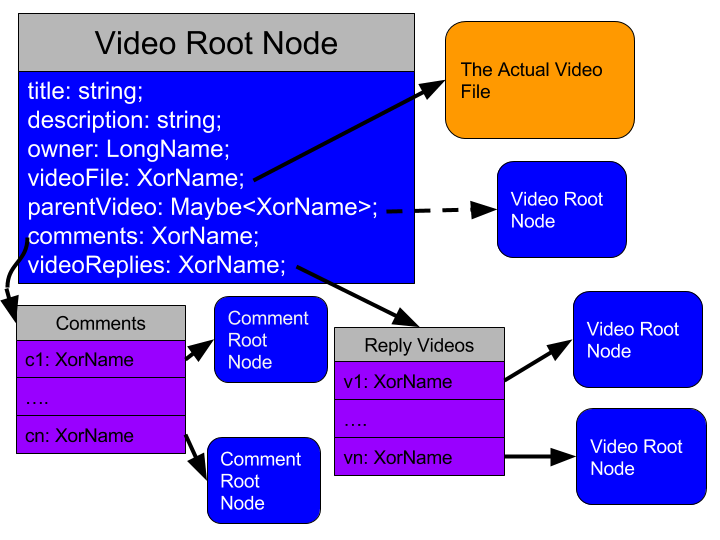
\includegraphics[width=0.8\linewidth]{video-model.png}
  \caption{Frames Video Model}
  \label{fig:video-model}
  \end{figure}

  The video model shown in figure \ref{fig:video-model} contains references to
  other videos as well as comments, and the owners of videos. References to videos and comments
  represented with an XorName, while references to owners of videos are
  represented with LongNames which make use of the SafeNET's identity system.

  \begin{figure}
  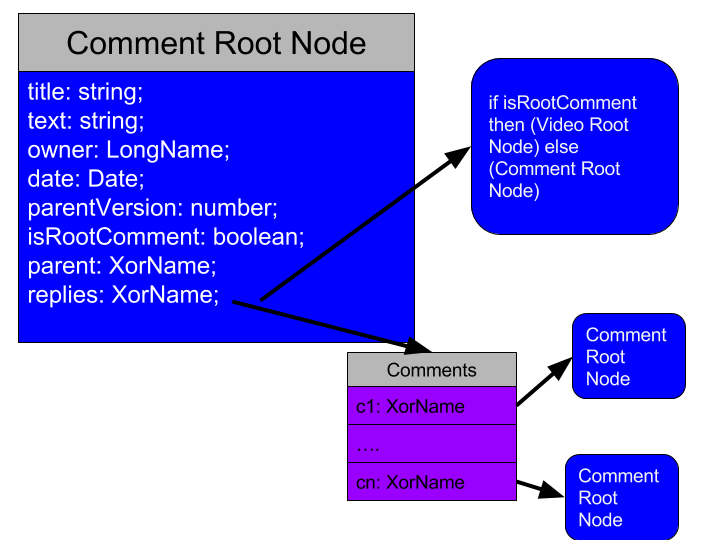
\includegraphics[width=0.8\linewidth]{comment-model.png}
  \caption{Frames Comment Model}
  \label{fig:comment-model}
  \end{figure}

\end{block}

%----------------------------------------------------------------------------------------

\end{column} % End of column 2.1

\begin{column}{\onecolwid}\vspace{-.6in} % The second column within column 2 (column 2.2)

%----------------------------------------------------------------------------------------

\begin{block}{}

  \begin{figure}
  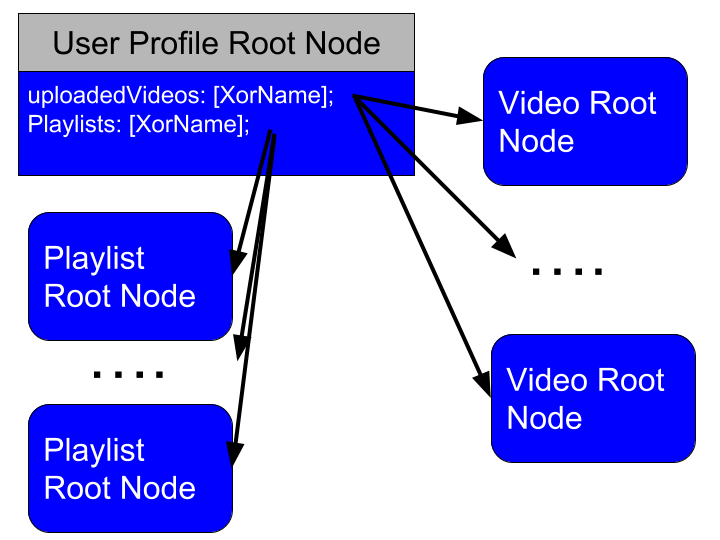
\includegraphics[width=0.8\linewidth]{user-profile-model.png}
  \caption{Frames UserProfile Model}
  \label{fig:user-profile-model}
  \end{figure}

  \begin{figure}
  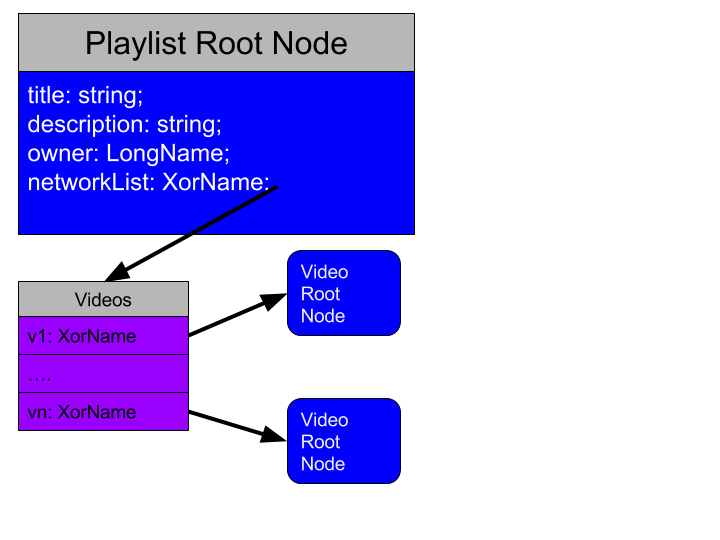
\includegraphics[width=0.8\linewidth]{playlist-model.png}
  \caption{Frames Playlist Model}
  \label{fig:playlist-model}
  \end{figure}

\end{block}

\begin{block}{Screen Shots}

  \begin{figure}
  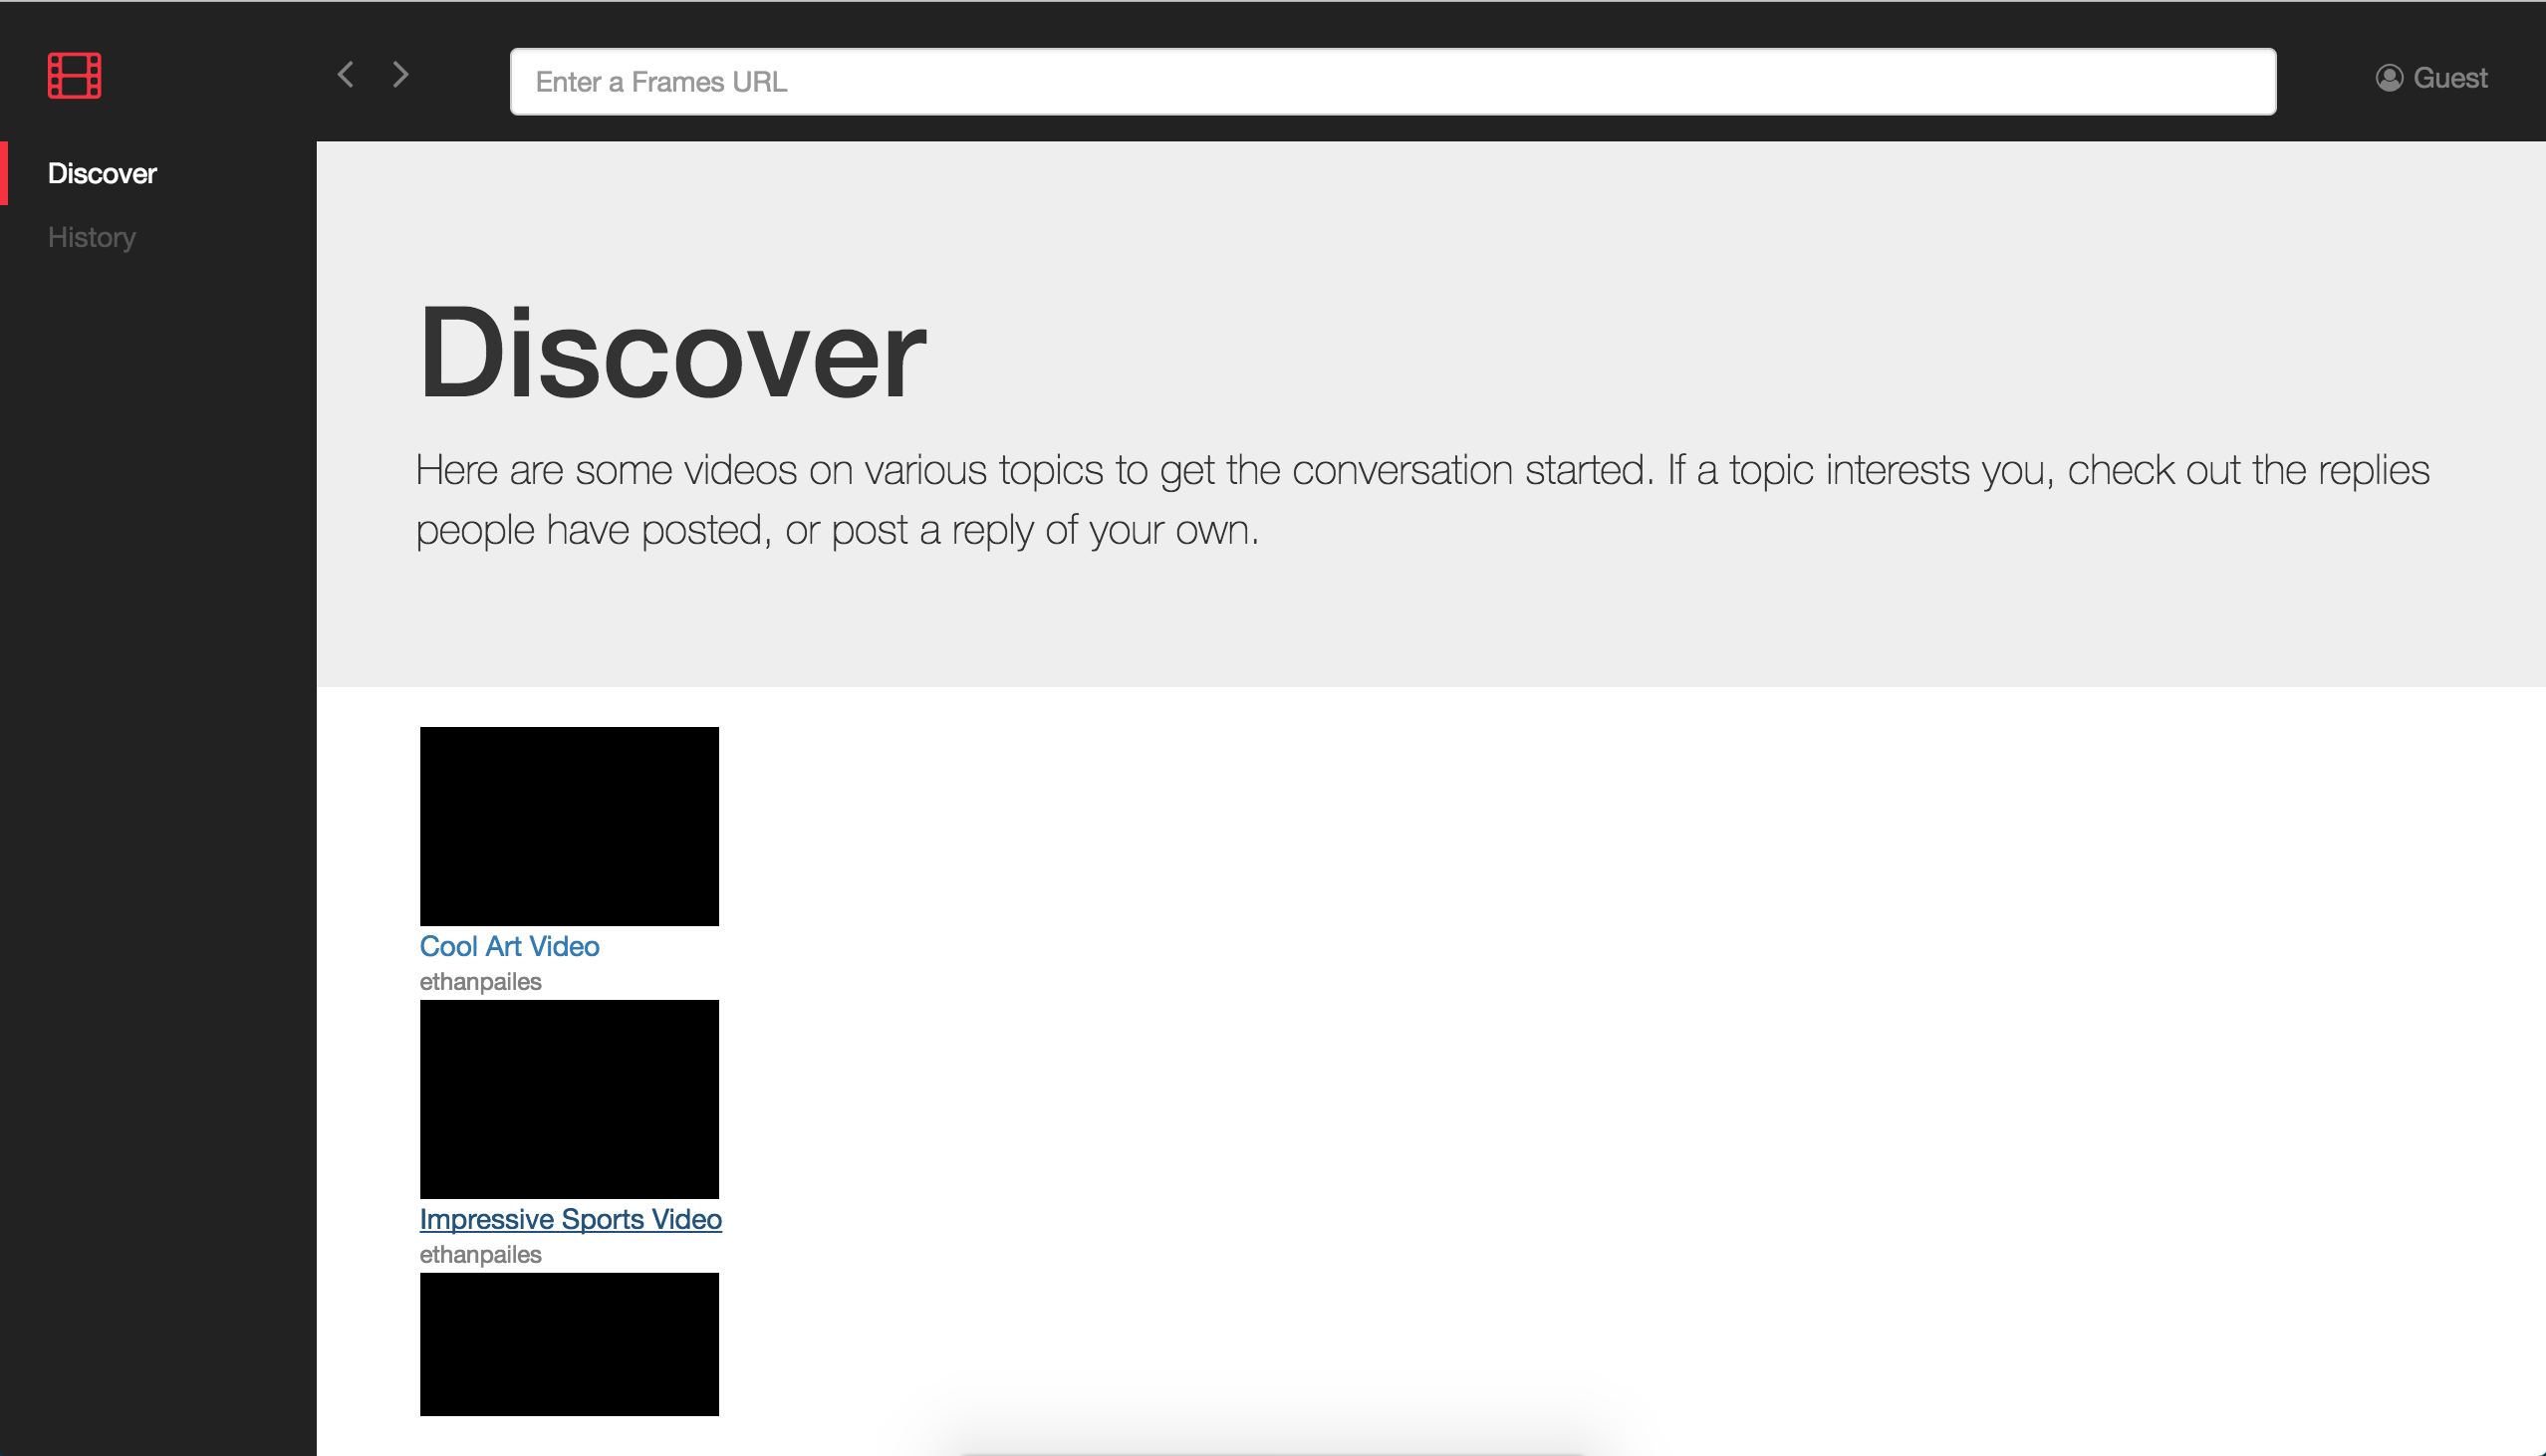
\includegraphics[width=0.8\linewidth]{discover-page.png}
  \captionsetup{labelformat=empty}
  \label{fig:discover-page}
  \end{figure}

\end{block}

\end{column} % End of column 2.2

\end{columns} % End of the split of column 2 - any content after this will now take up 2 columns width

%----------------------------------------------------------------------------------------

\begin{columns}[t,totalwidth=\twocolwid] % Split up the two columns wide column again


\end{columns} % End of the split of column 2

\end{column} % End of the second column

\begin{column}{\sepwid}\end{column} % Empty spacer column

\begin{column}{\onecolwid} % The third column

%----------------------------------------------------------------------------------------
%	CONCLUSION
%----------------------------------------------------------------------------------------

\begin{block}{}

  \begin{figure}
  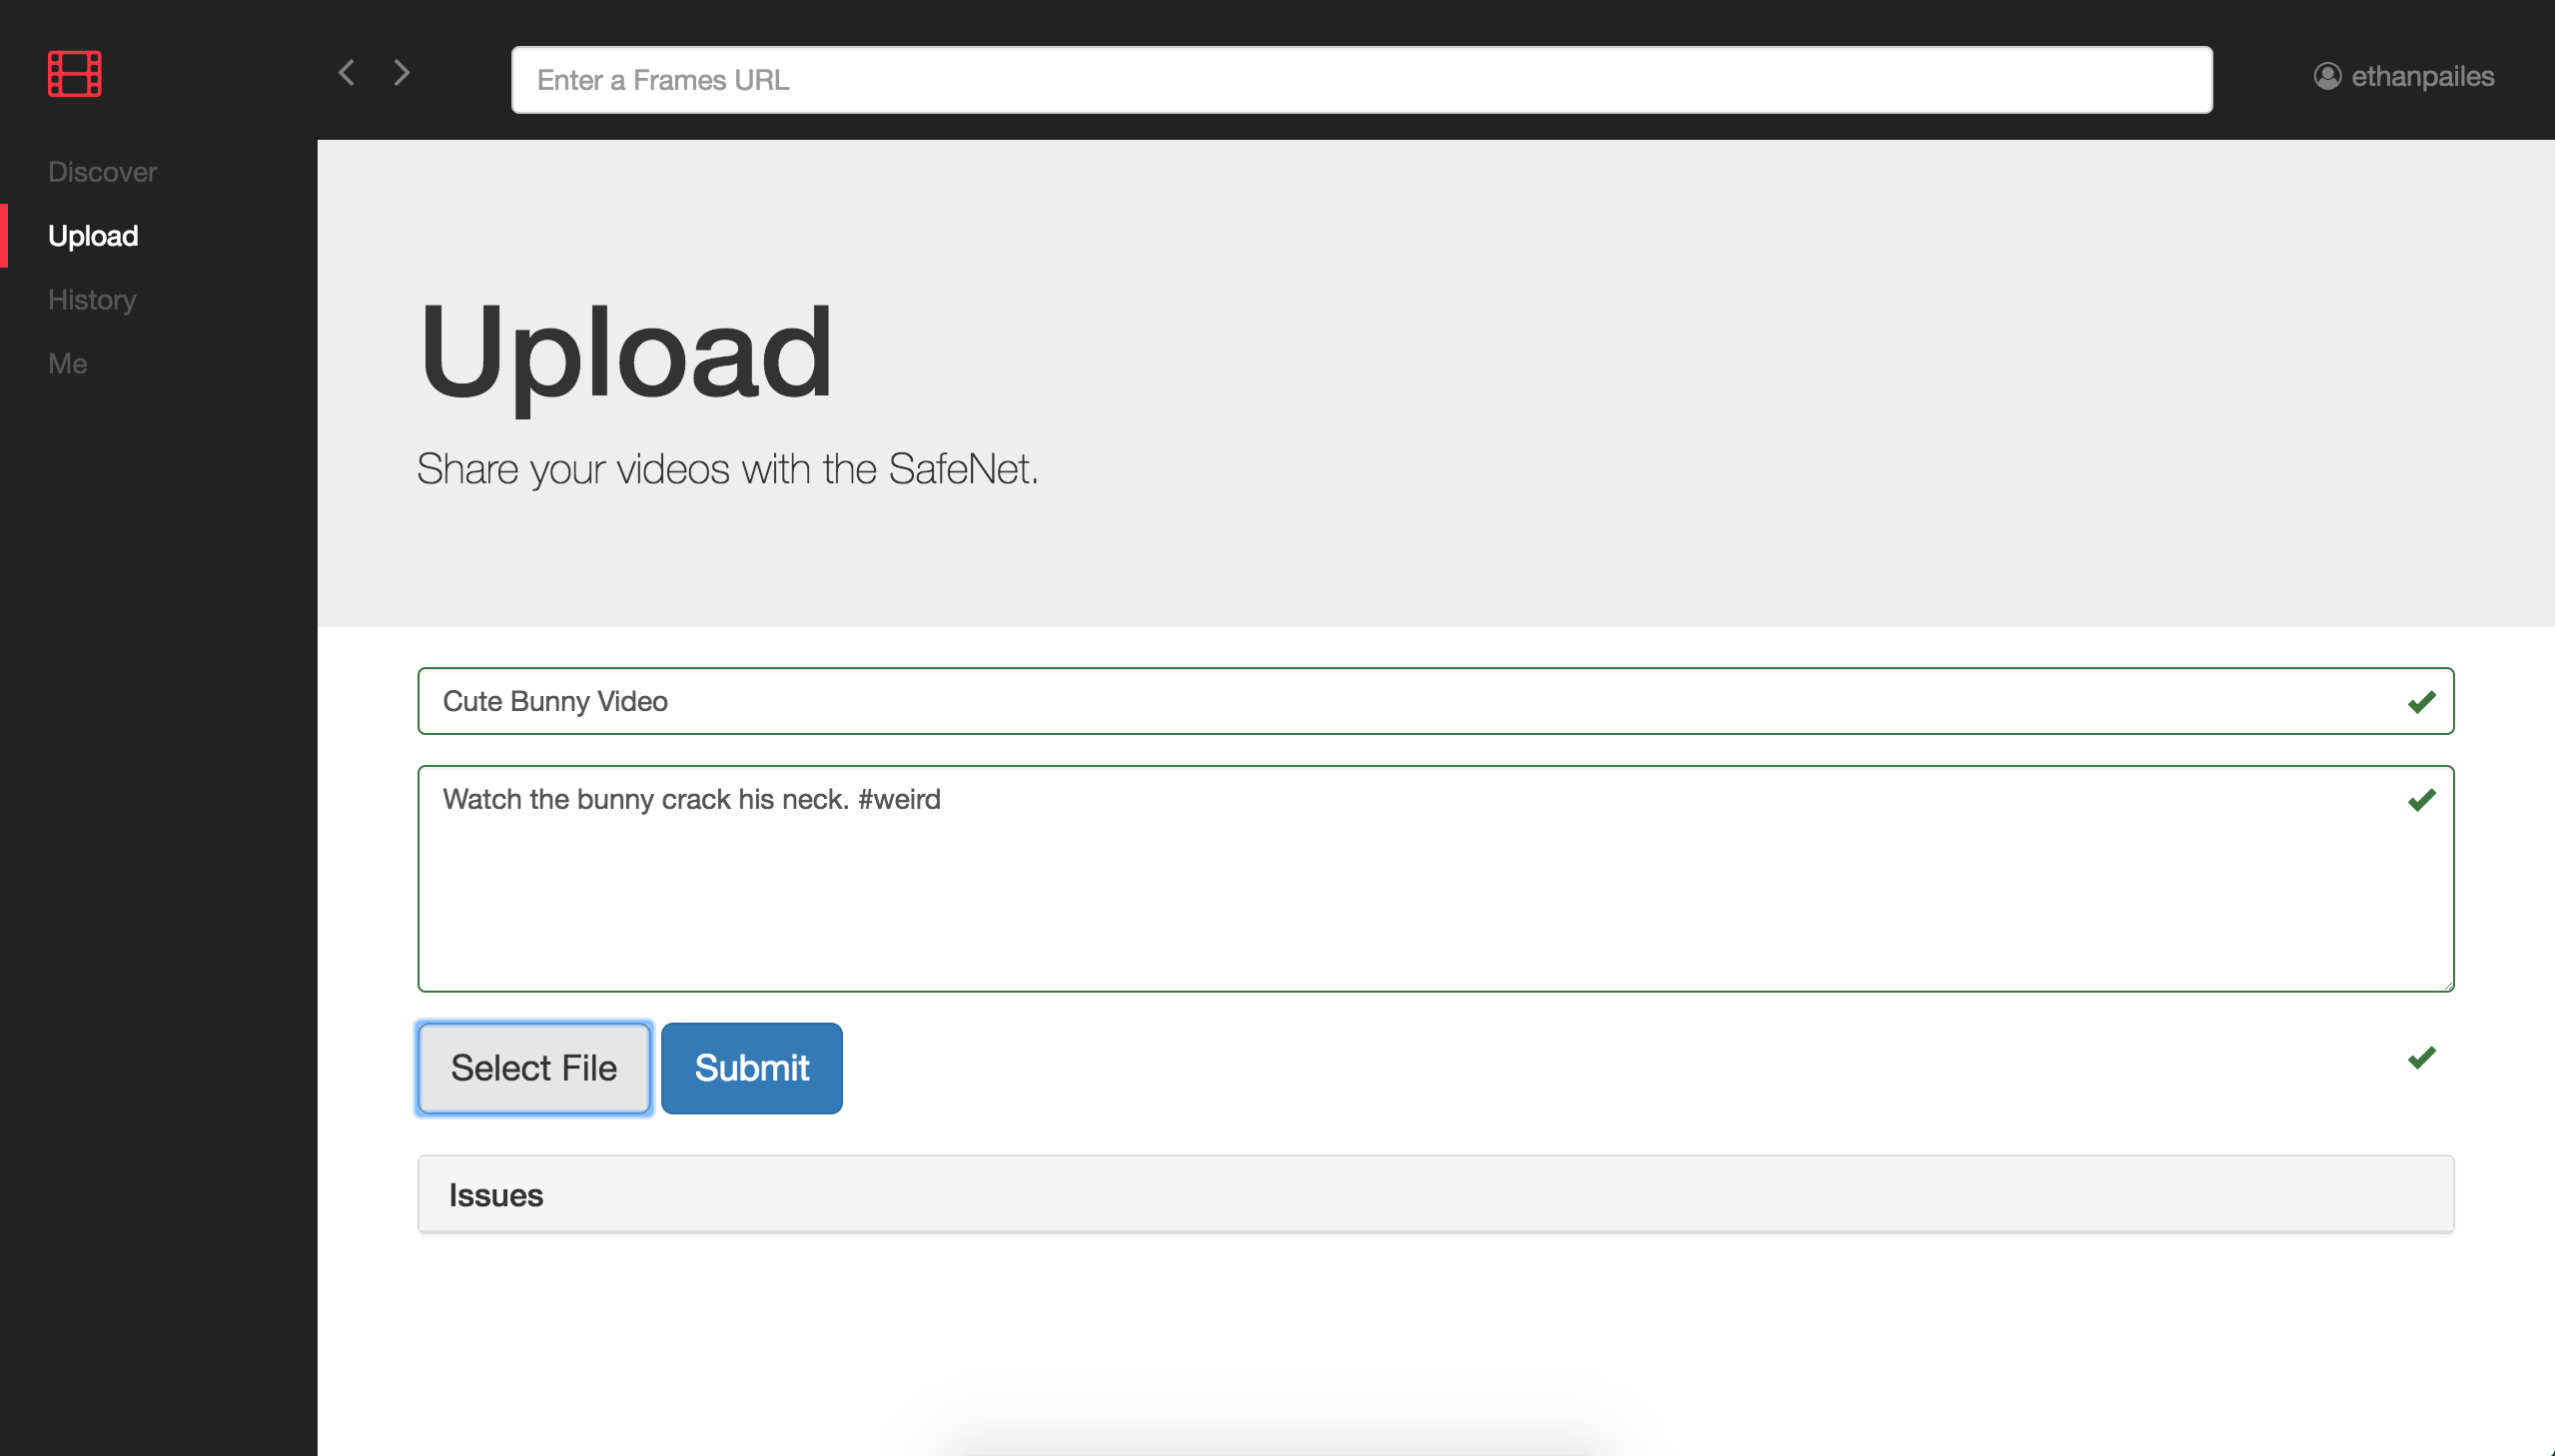
\includegraphics[width=0.8\linewidth]{upload-page.png}
  \captionsetup{labelformat=empty}
  \label{fig:upload-page}
  \end{figure}

  \begin{figure}
  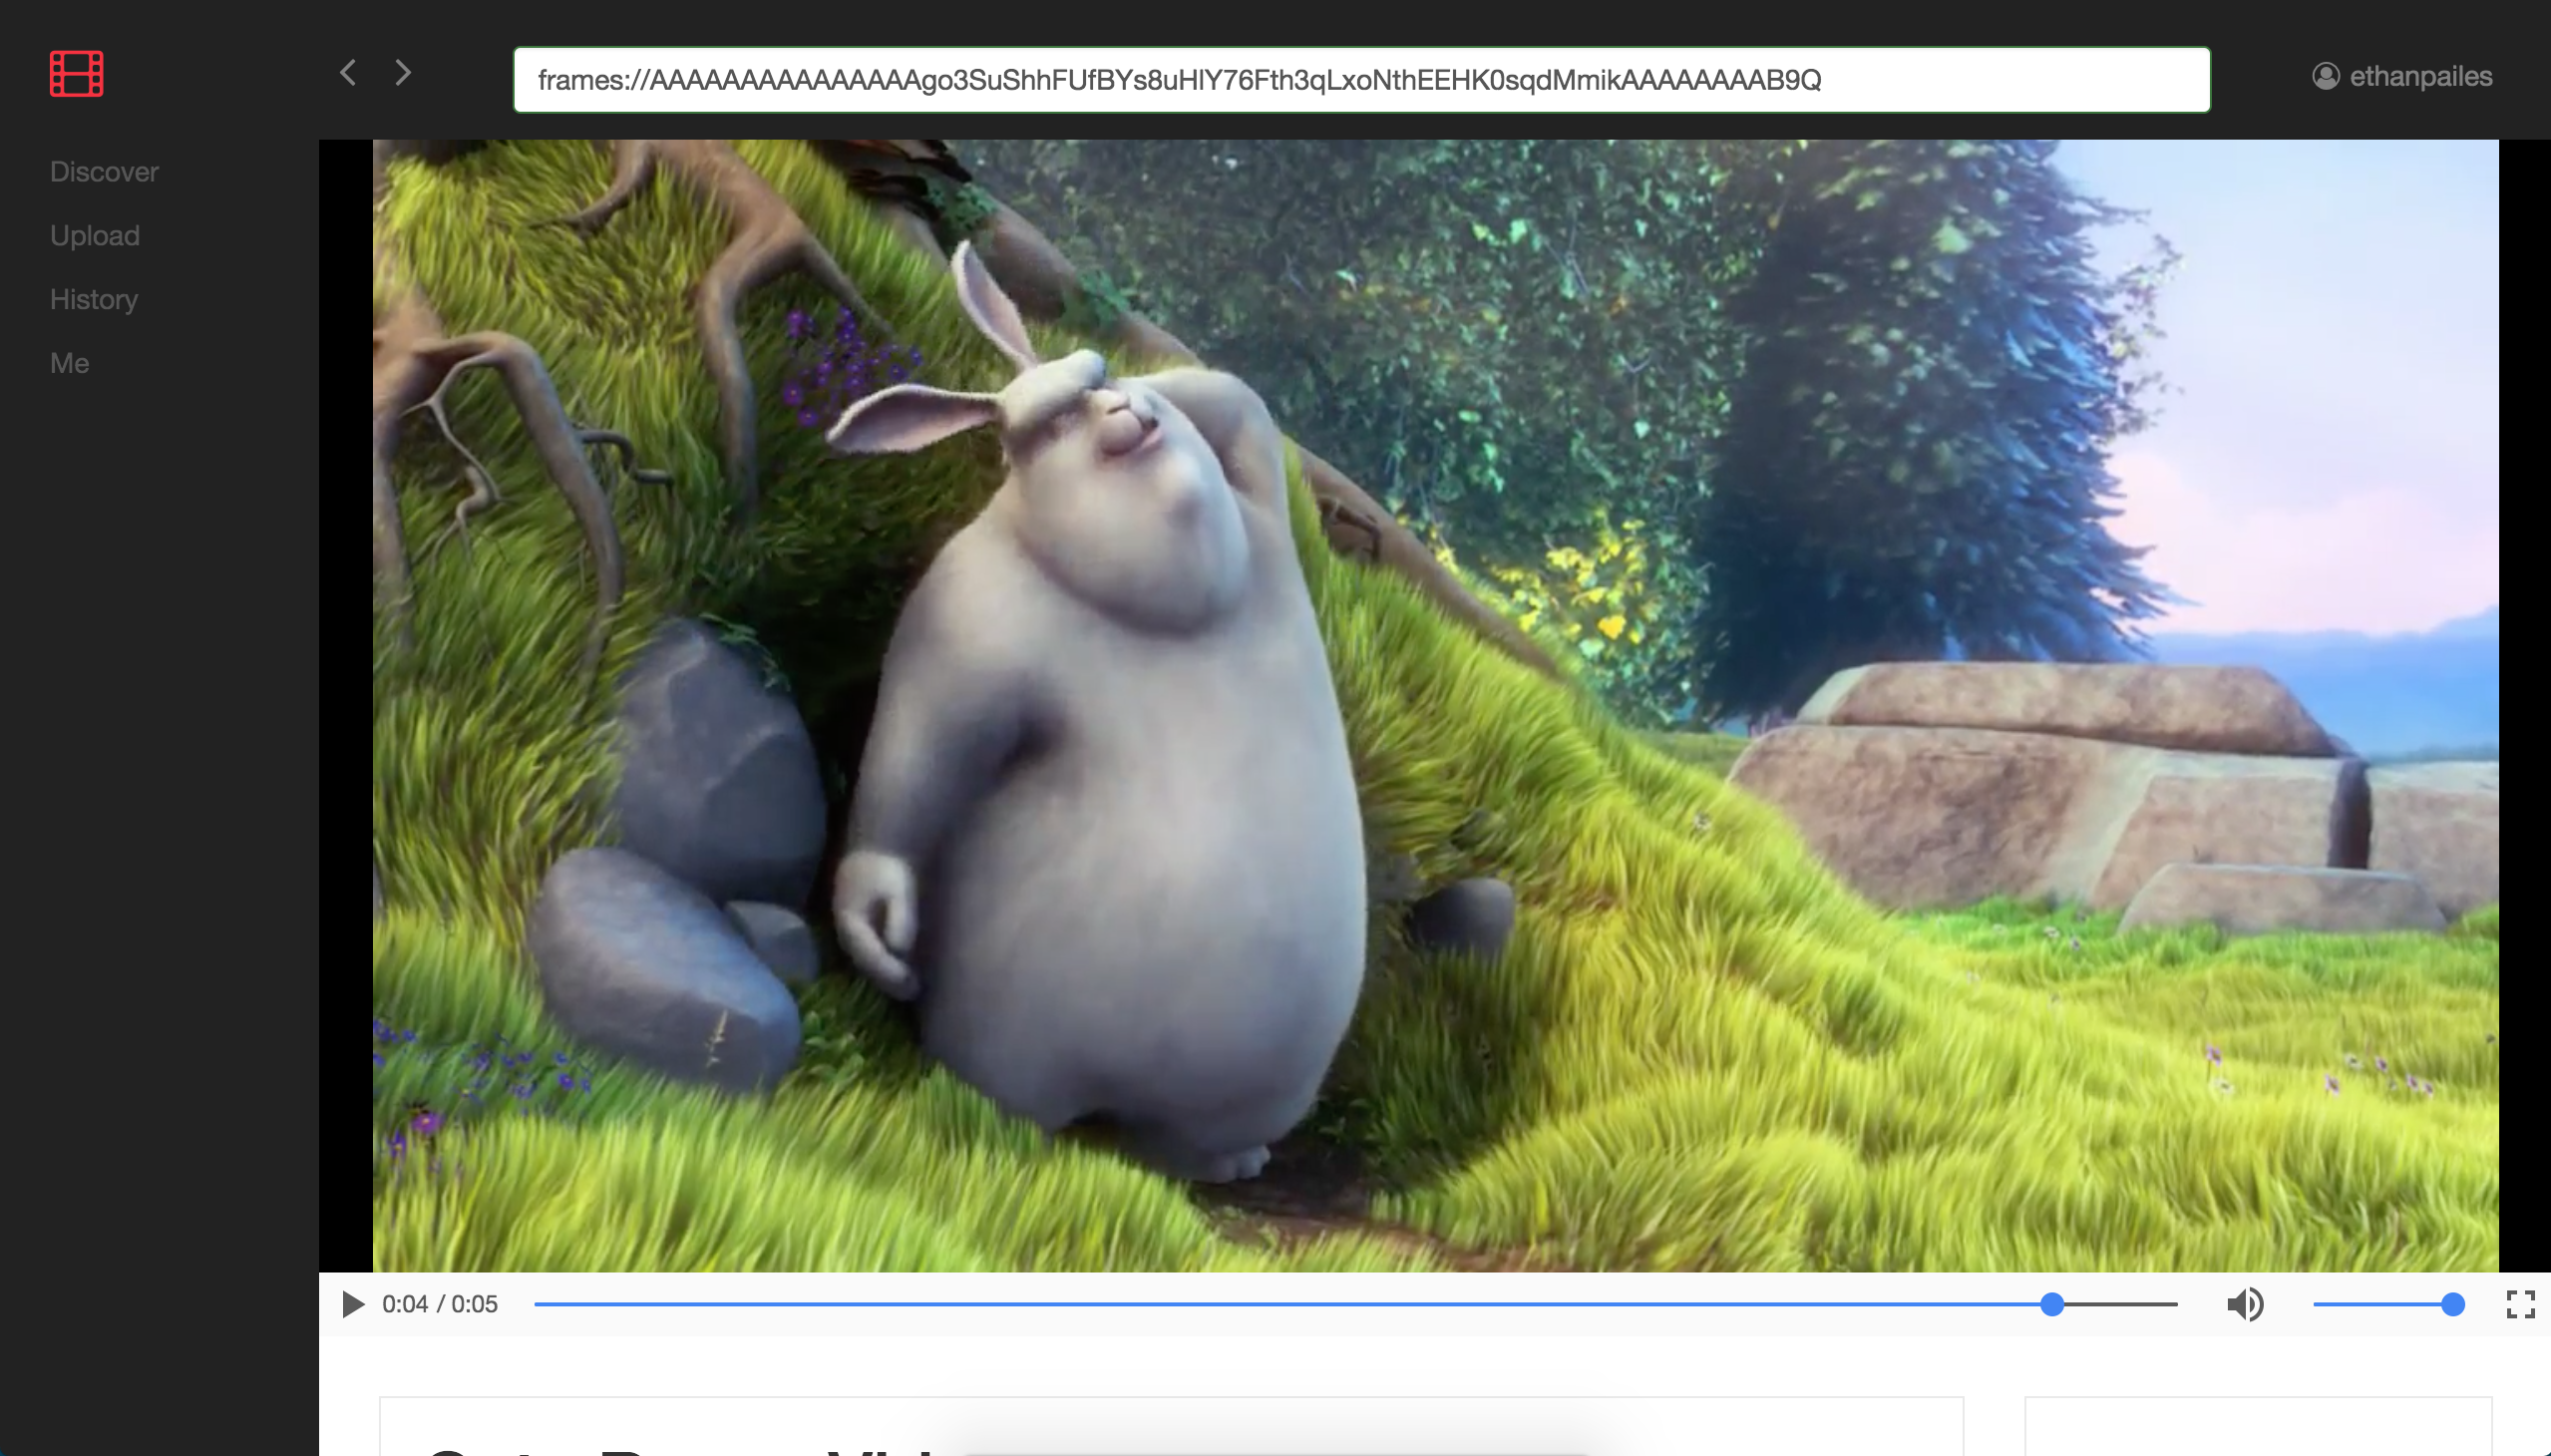
\includegraphics[width=0.8\linewidth]{watch-page.png}
  \captionsetup{labelformat=empty}
  \label{fig:watch-page}
  \end{figure}

  \begin{figure}
  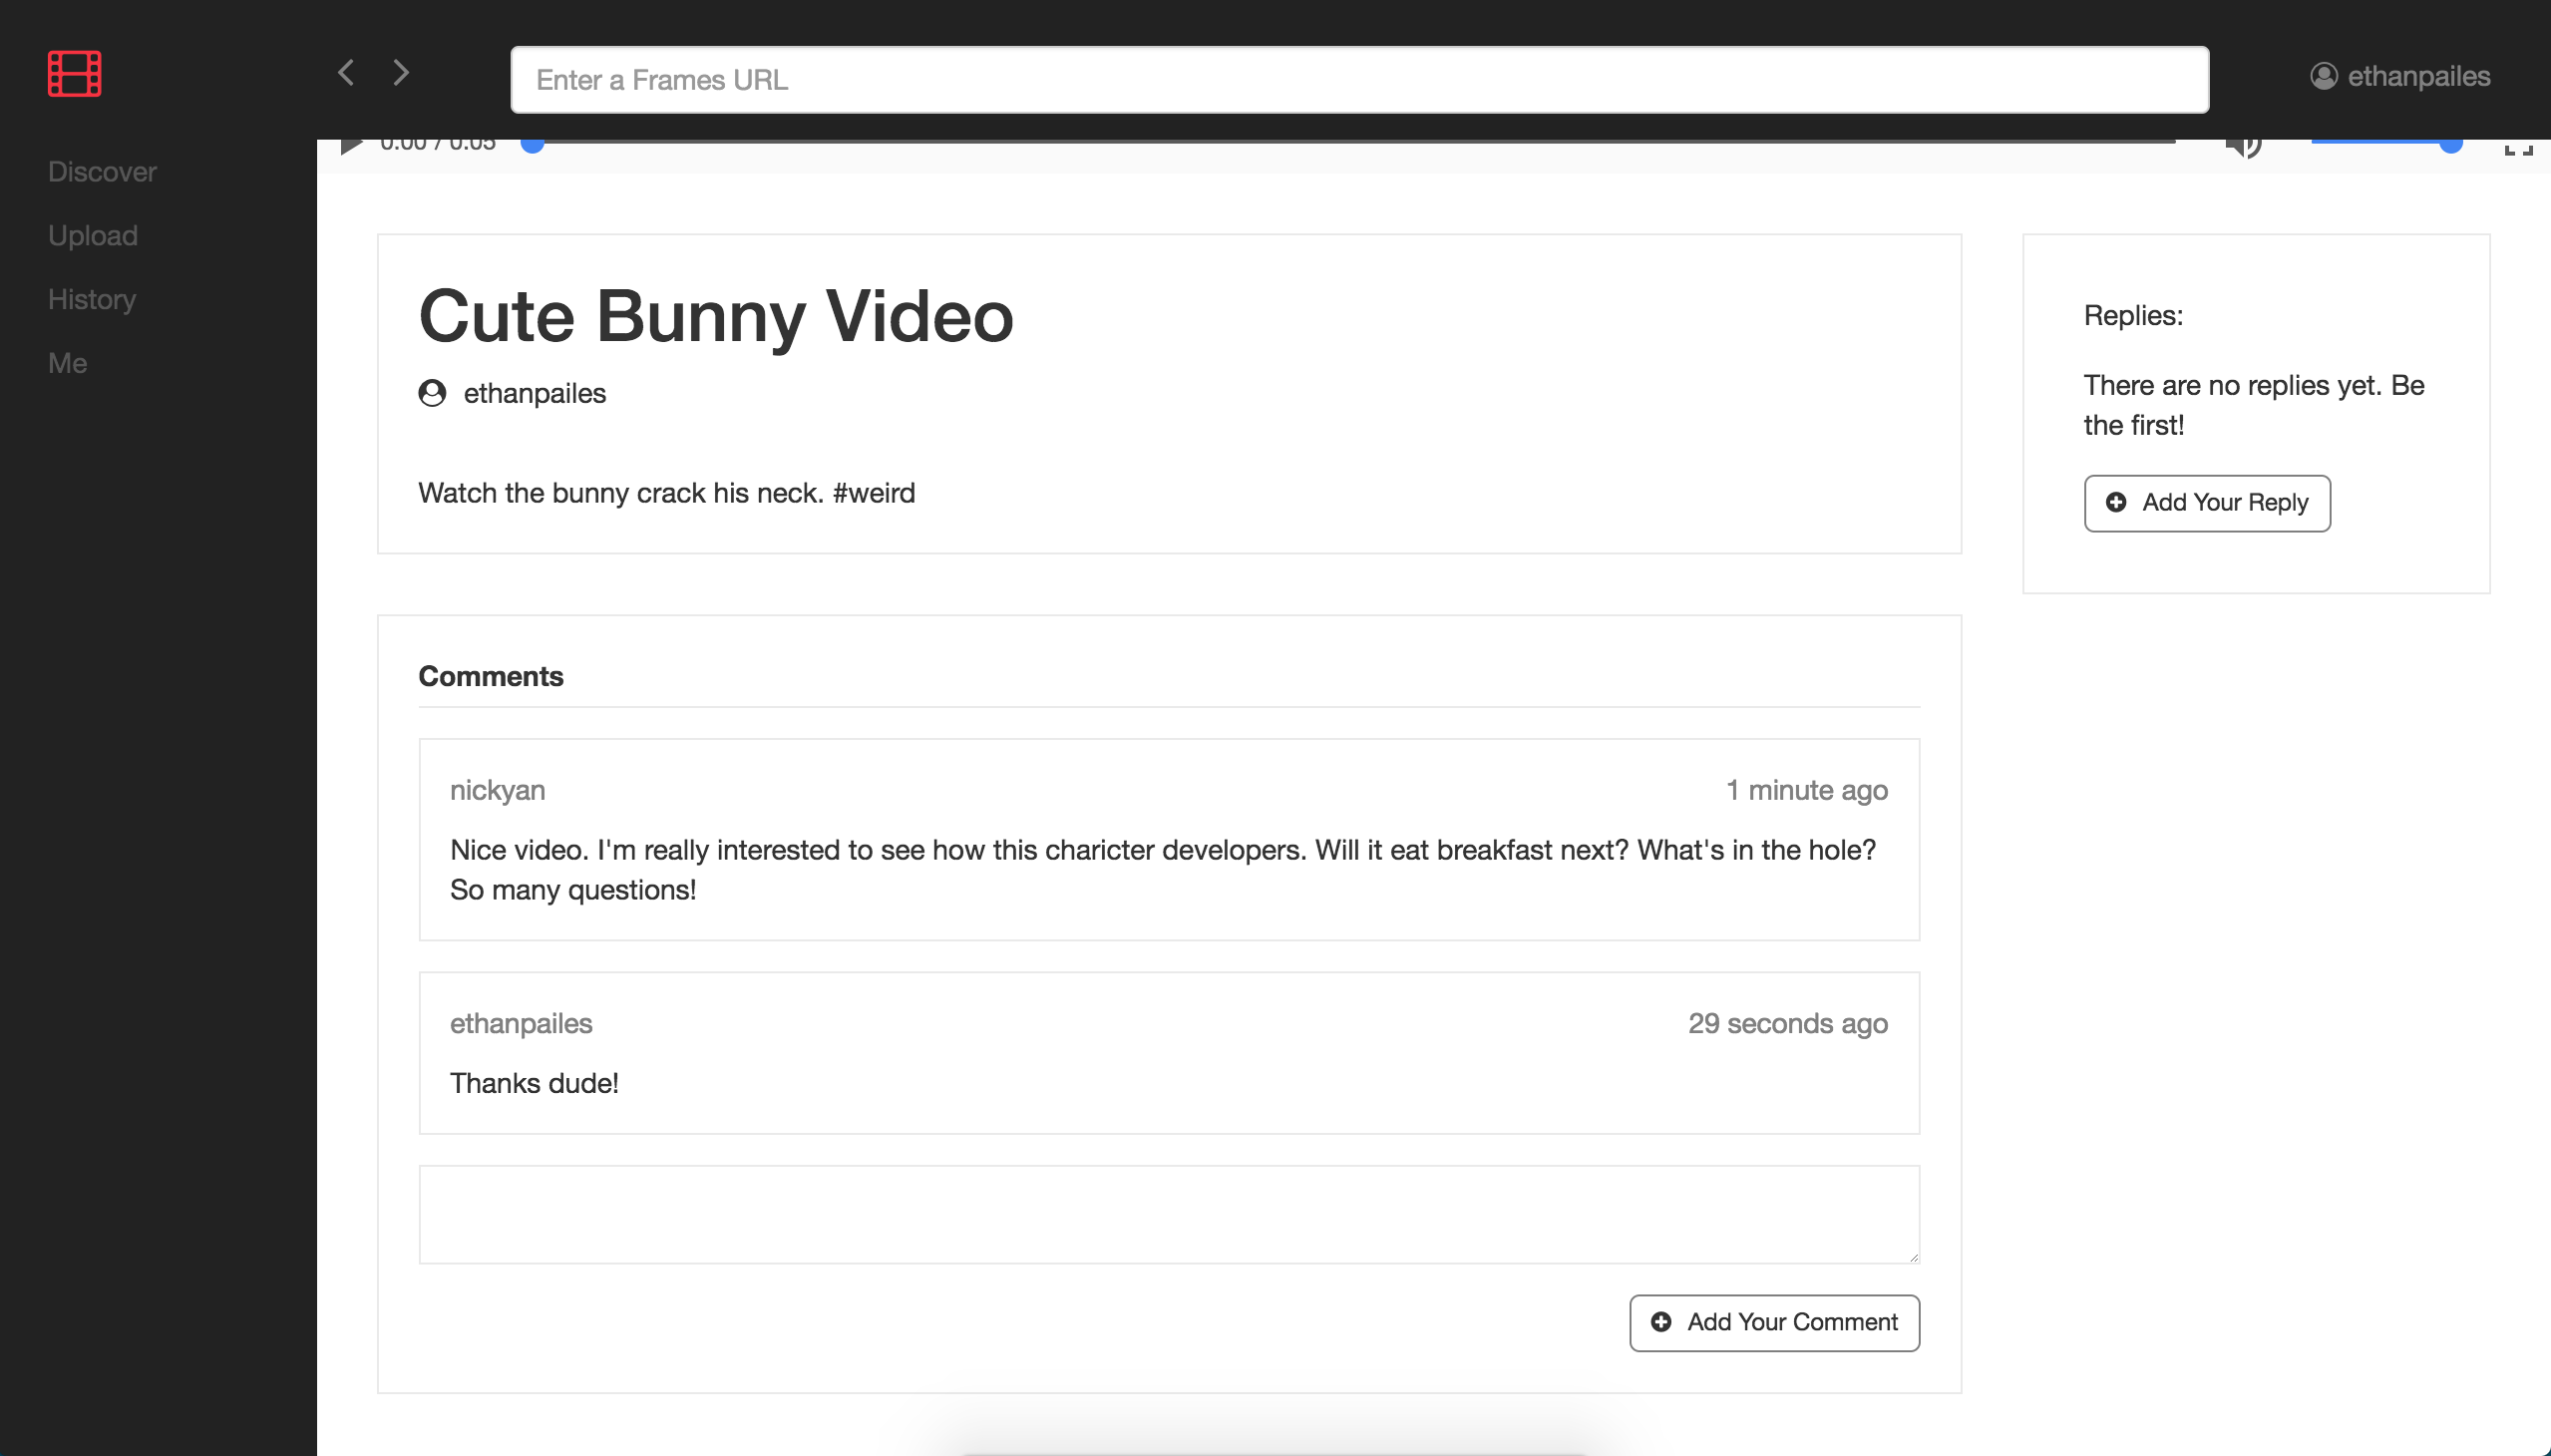
\includegraphics[width=0.8\linewidth]{watch-page-comments.png}
  \captionsetup{labelformat=empty}
  \label{fig:watch-page-comments}
  \end{figure}

\end{block}


%----------------------------------------------------------------------------------------
%	ACKNOWLEDGEMENTS
%----------------------------------------------------------------------------------------

\setbeamercolor{block title}{fg=red,bg=white} % Change the block title color

\begin{block}{Acknowledgements}

\small{\rmfamily{Nam mollis tristique neque eu luctus. Suspendisse rutrum congue nisi sed convallis. Aenean id neque dolor. Pellentesque habitant morbi tristique senectus et netus et malesuada fames ac turpis egestas.}} \\

\end{block}

%----------------------------------------------------------------------------------------

\end{column} % End of the third column

\end{columns} % End of all the columns in the poster

\end{frame} % End of the enclosing frame

\end{document}

